\title{Taysols\\ ML model \\ train and deploy model Batch}
\author{Yiran Jing 
}
\date{June, 2019}
\documentclass[12pt]{article}
\usepackage[toc,page]{appendix}
\usepackage{graphicx} 
\usepackage{float}
\usepackage{caption}
\usepackage{subcaption}
\usepackage{geometry}
\usepackage{amsmath}
\usepackage{lscape}
\usepackage{natbib}
\usepackage{adjustbox}
\usepackage{changepage}
\usepackage{multicol}
\usepackage{booktabs}
\usepackage{hyperref}


\usepackage[dvipsnames]{xcolor}
\definecolor{mypink1}{rgb}{0.858, 0.188, 0.478}
\definecolor{mypink2}{cmyk}{0, 0.7808, 0.4429, 0.1412}
\definecolor{mygray}{gray}{0.6}
\colorlet{myorange}{green!10!orange!90!}

\geometry{
	a4paper,
	total={170mm,257mm},
	left=25mm,
	right=25mm,
	top=25mm,
	bottom=20mm}

\newcommand{\HRule}[1]{\rule{\linewidth}{#1}}
\setcounter{tocdepth}{5}
\setcounter{secnumdepth}{5}

\begin{document}

\title{ \normalsize \textsc{Data Science}
		\\ [2.0cm]
		\HRule{0.5pt} \\
		\LARGE \textbf{\uppercase{Churn Prediction with buildin Sagemaker XGBoost}}
		\HRule{2pt} \\ [0.5cm]
		\small \textbf{Amazon SageMaker: Train and Deploy build-in XGBoost with Batch Transform}
		\normalsize \vspace*{5\baselineskip}}
		
\date{July 02, 2019}
\author{Yiran Jing\\}
\maketitle

\pagenumbering{gobble}
\newpage
\thispagestyle{empty}


\newpage
\tableofcontents
\newpage
\setcounter{page}{1}
\pagenumbering{arabic}
\section{Dataset description}

The customer churn dataset includes 7021 customers (after remove duplicates) with 20 features, and target column is churn. Since the origin data is dirty with missing values and apparently wrong records, I clean the dataset before the following steps. 
Look \href{https://github.com/YiranJing/BigDataAnalysis/blob/master/AWS_SageMaker_CustomerChurn/notebook/ChurnDataAnalysis/Churn_Example.ipynb}{\textbf{Churn example} (\textit{Click me to open this notebook})} for details about clean data and feature engineering.
\\

\noindent
Amazon SageMaker XGBoost can train on data in either a CSV or LibSVM format. For this example, we use CSV. It should have the following:
\begin{enumerate}
\item Have the predictor variable in the first column (as per AWS requirements)
\item Not have a header row (as per AWS requirements)
\item No customer\_id (Useless column)
\item Numerical entry only (cleaned dataset as per AWS requirements)

\end{enumerate}



\noindent
\textbf{Data Description} :We need four datasets (you can find them in S3 churn buckets):
\begin{enumerate}
\item train.csv (70\%) (include target) 

\item validation.csv (20\%) (include target) \textit{: validation is the test dataset despite the confusing name}

\item test.csv (10\%) (include target) \textit{: is for evaluating the model once deployed} 

\item test\_data\_Batch.csv (10\%) (remove the target column from test.csv) 
\end{enumerate} 


\noindent
In \textit{train.csv}, \textit{validation.csv}, and \textit{test.csv}, the \textbf{first column is target}, and \textbf{no header}, also removed column \textit{customer\_id}, and the dataset contain \textbf{numerical entry only}. Based on the input data format of Batch transformation, I create \textit{test\_data\_Batch.csv} dataset, which contain the same predictors information with \textit{test.csv}, but remove the target column.
\\

\noindent
The test data prediction will be in \textbf{\textit{test\_data\_Batch.csv.out}} after batch transformation. It gives the probability for each observation in test dataset. 

\noindent
Also, you can check the output file once training is finished 


\newpage
\section{Train Model}
All following code screenshots are from \href{https://github.com/YiranJing/BigDataAnalysis/blob/master/AWS_SageMaker_CustomerChurn/notebook/AmazonSageMaker/AWS_BUILTIN_MODEL_DEPLOYMENT.ipynb}{(\textit{Click me to open this notebook})}.
\\

\noindent
We need two dataset \textit{train.csv} and \textit{validation.csv} for training model.

\subsection{Set role and model container}
See figure \ref{fig:set_role_container}, the first step we need to do is get execution role and get the XGBoost container. You can paste the following code in a cell in the Jupyter notebook you created for any XGBoost modelling.

\begin{figure}[H]
\centering
\begin{minipage}{1\textwidth}
  \centering
  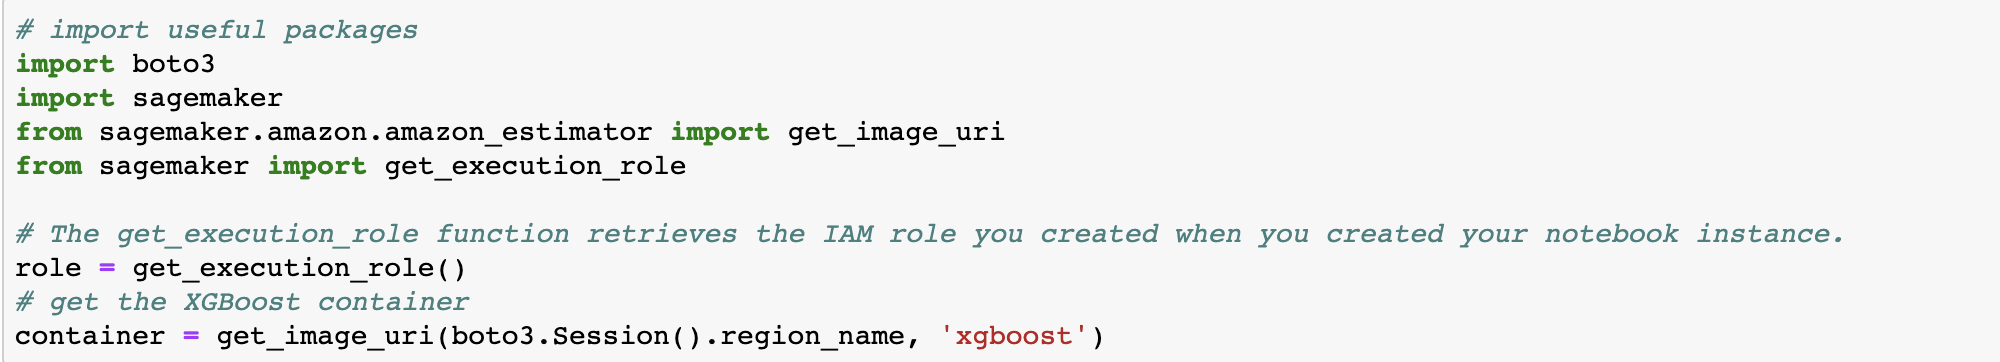
\includegraphics[width=1\linewidth]{set_role_container.png}
   \caption{Input package, set role and model container}
   \label{fig:set_role_container}
\end{minipage}%
\end{figure}

\subsection{Read in train and validation data from S3 bucket}
See figure \ref{fig:set_data_path}, the second step is find the data path and then read in train and validation data. Note that we \textbf{must have two data files train file and validation file, and only one csv dataset in each data file}. We cannot specify the name of train or validation dataset, but we need to specify the dataset type (csv in our case). That is,
$$s3\_input\_train = bucket/prefix/train/$$ any CSV dataset with in train file will be read as train data, note that \textbf{Only one csv datafile} shall be put in train data file. Same as validation file. In my example, the bucket's name is taysolsdev. When you first time try training model on AWS, the main challenge might be finding out the correct path (i.e. name of bucket and prefix). Well the following steps will be pretty easy after you finding out this.

\begin{figure}[H]
\centering
\begin{minipage}{1\textwidth}
  \centering
  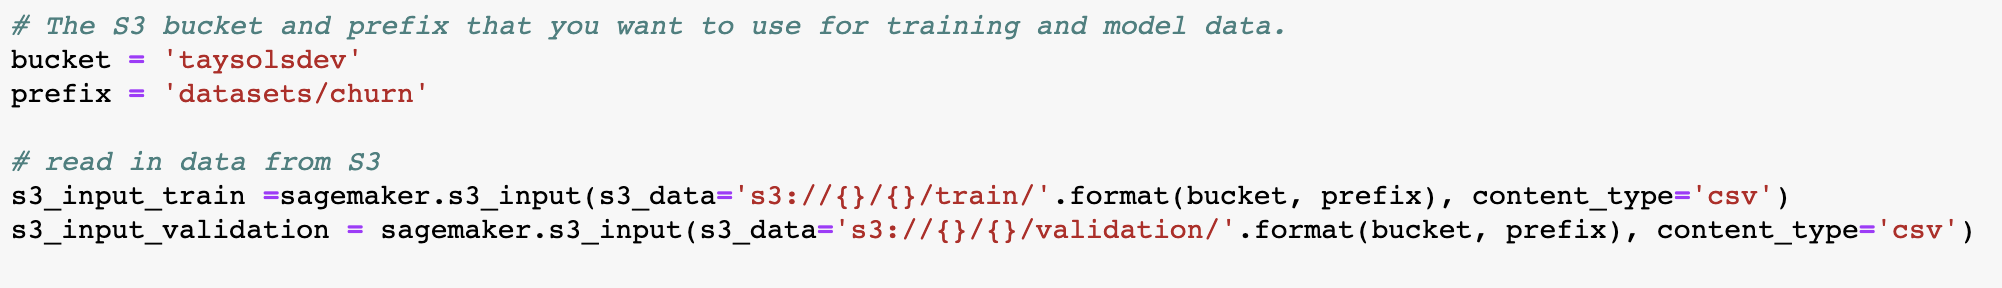
\includegraphics[width=1\linewidth]{set_data_path.png}
   \caption{Read data from S3 bucket}
   \label{fig:set_data_path}
\end{minipage}%
\end{figure}

\subsection{Specific Output path and Create estimator instance}
See figure \ref{fig:create_estimator_instance}, firstly, we create session object, and then create the estimator instance. Note that we need to give the output file path here. You can paste the following code in a cell in the Jupyter notebook 
\begin{figure}[H]
\centering
\begin{minipage}{1\textwidth}
  \centering
  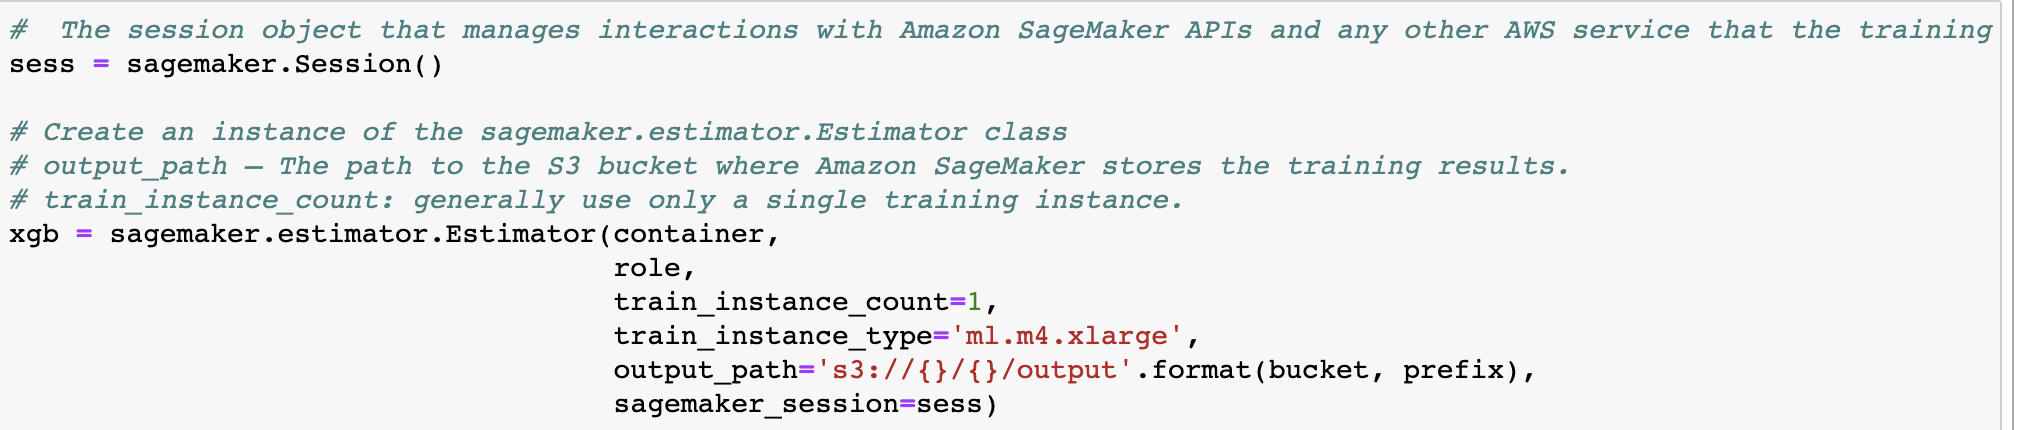
\includegraphics[width=1\linewidth]{create_estimator_instance.png}
   \caption{Create estimator instance}
   \label{fig:create_estimator_instance}
\end{minipage}%
\end{figure}
\noindent
 
\subsection{Set hyperparameter for GXBoost}
See figure \ref{fig:set_hypterparameter}, before actually train model, we can set optiminal hyperparameter in this step. Note that \textbf{\textit{silent} parameter must be integer}, cannot be none. And we \textbf{must set parameter \textit{num\_round}} in this step.
\\
\noindent
You can change \textbf{objective} parameter if use GXBoost for regression or multi-classification. Since our case is binary classification, I use \textit{binary:logistic}, and output is probability for each observation.

\begin{figure}[H]
\centering
\begin{minipage}{1\textwidth}
  \centering
  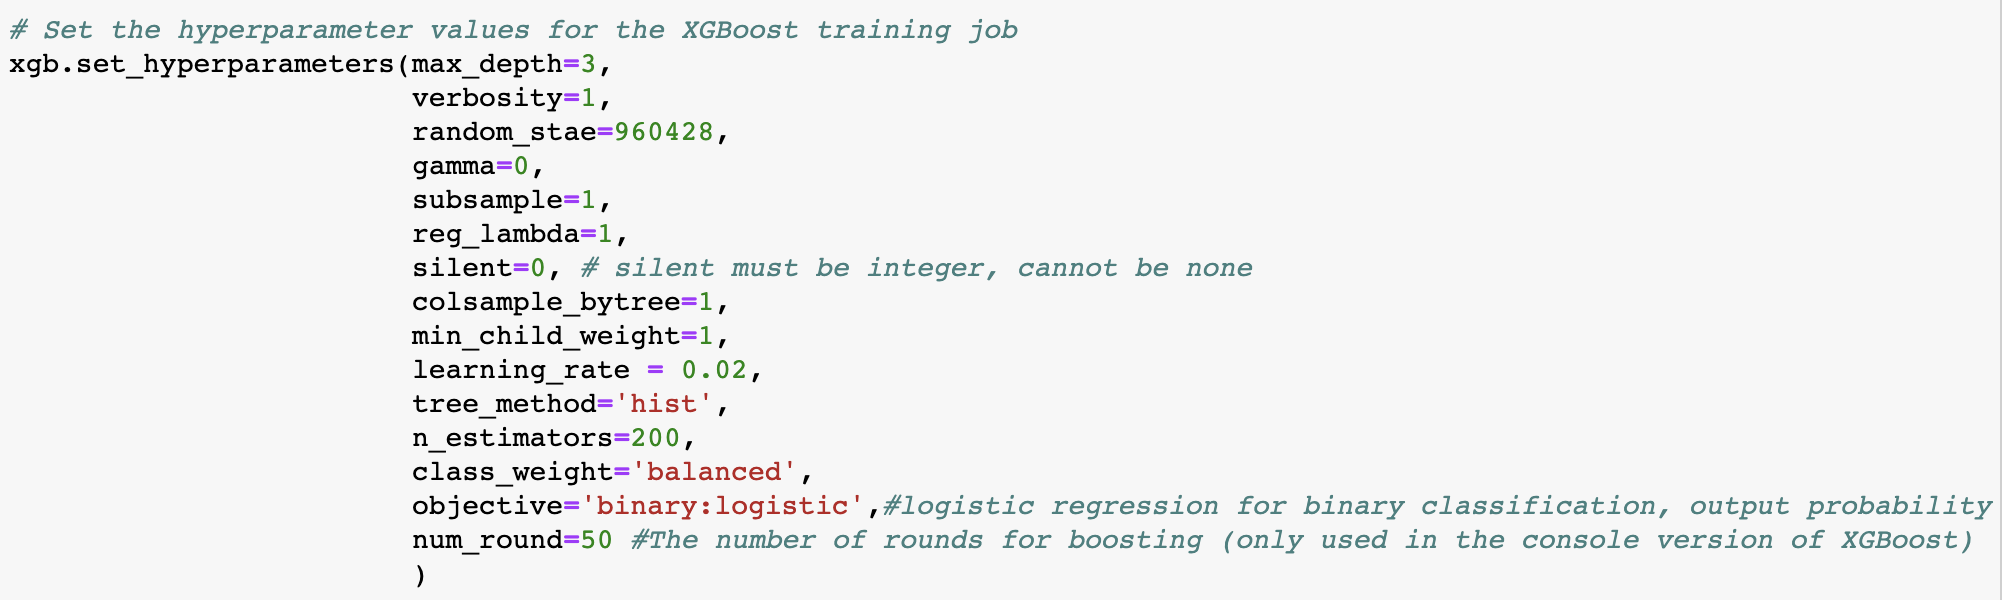
\includegraphics[width=1\linewidth]{set_hypterparameter.png}
   \caption{Set hyperparameter for GXBoost}
   \label{fig:set_hypterparameter}
\end{minipage}%
\end{figure}
\noindent

\subsection{Begin train model}
See figure \ref{fig:model_train}, since sagemaker uses \textbf{lazy evaluation}, we can only actually begin train model when we call \textit{.fit()} method. You can check the S3 output dataset with in output file after training job finish. You can paste the following code in a cell in the Jupyter notebook.
\begin{figure}[H]
\centering
\begin{minipage}{1\textwidth}
  \centering
  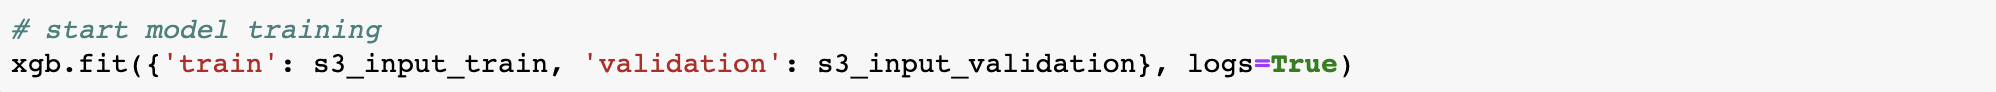
\includegraphics[width=1\linewidth]{model_train.png}
   \caption{Begin train model}
   \label{fig:model_train}
\end{minipage}%
\end{figure}
\noindent


\subsection{Another way to train model: SDK format}
\textbf{JSON format for configuring model}: The version in this section follows the SDK format that calls to the AWS API for building an ML model. Another way to do this would be to configure the model using JSON format as below.

\subsubsection{User-defined Model name}
In this method, since we need to configuring model, we need to know the name of the model we are running, and we can also define the model name by ourselves. You are open Amazon SamgeMaker interface to check the model name. 
\begin{figure}[H]
\centering
\begin{minipage}{1\textwidth}
  \centering
  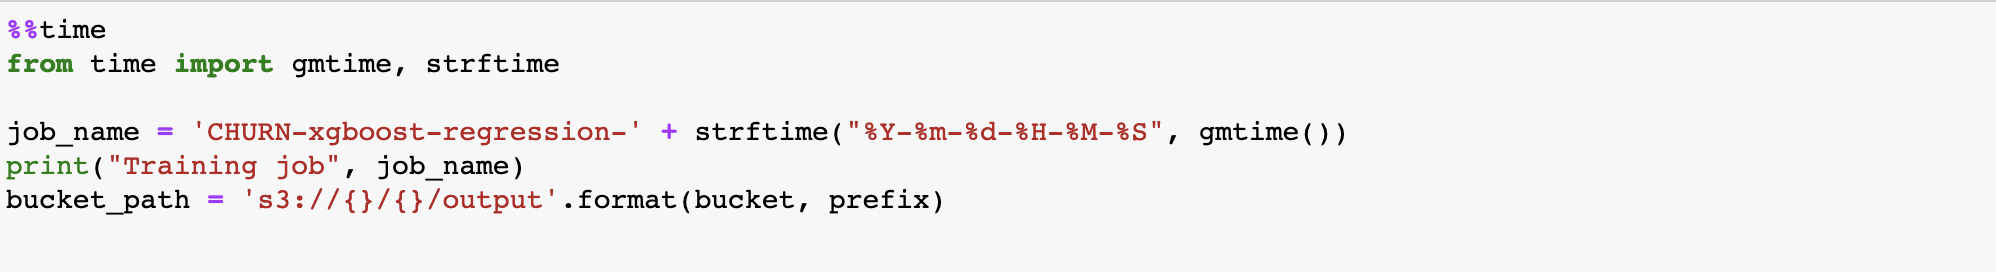
\includegraphics[width=1\linewidth]{UDModel_name.png}
   \caption{User-defined Model name}
   \label{fig:UDModel_name}
\end{minipage}%
\end{figure}
\noindent

\subsubsection{configuring model}
Ensure that the training and validation data folders generated above are reflected in the \textbf{InputDataConfig} parameter below. See figure \ref{fig:confgi_1} and figure \ref{fig:confgi_2}:
\begin{figure}[H]
\centering
\begin{minipage}{1\textwidth}
  \centering
  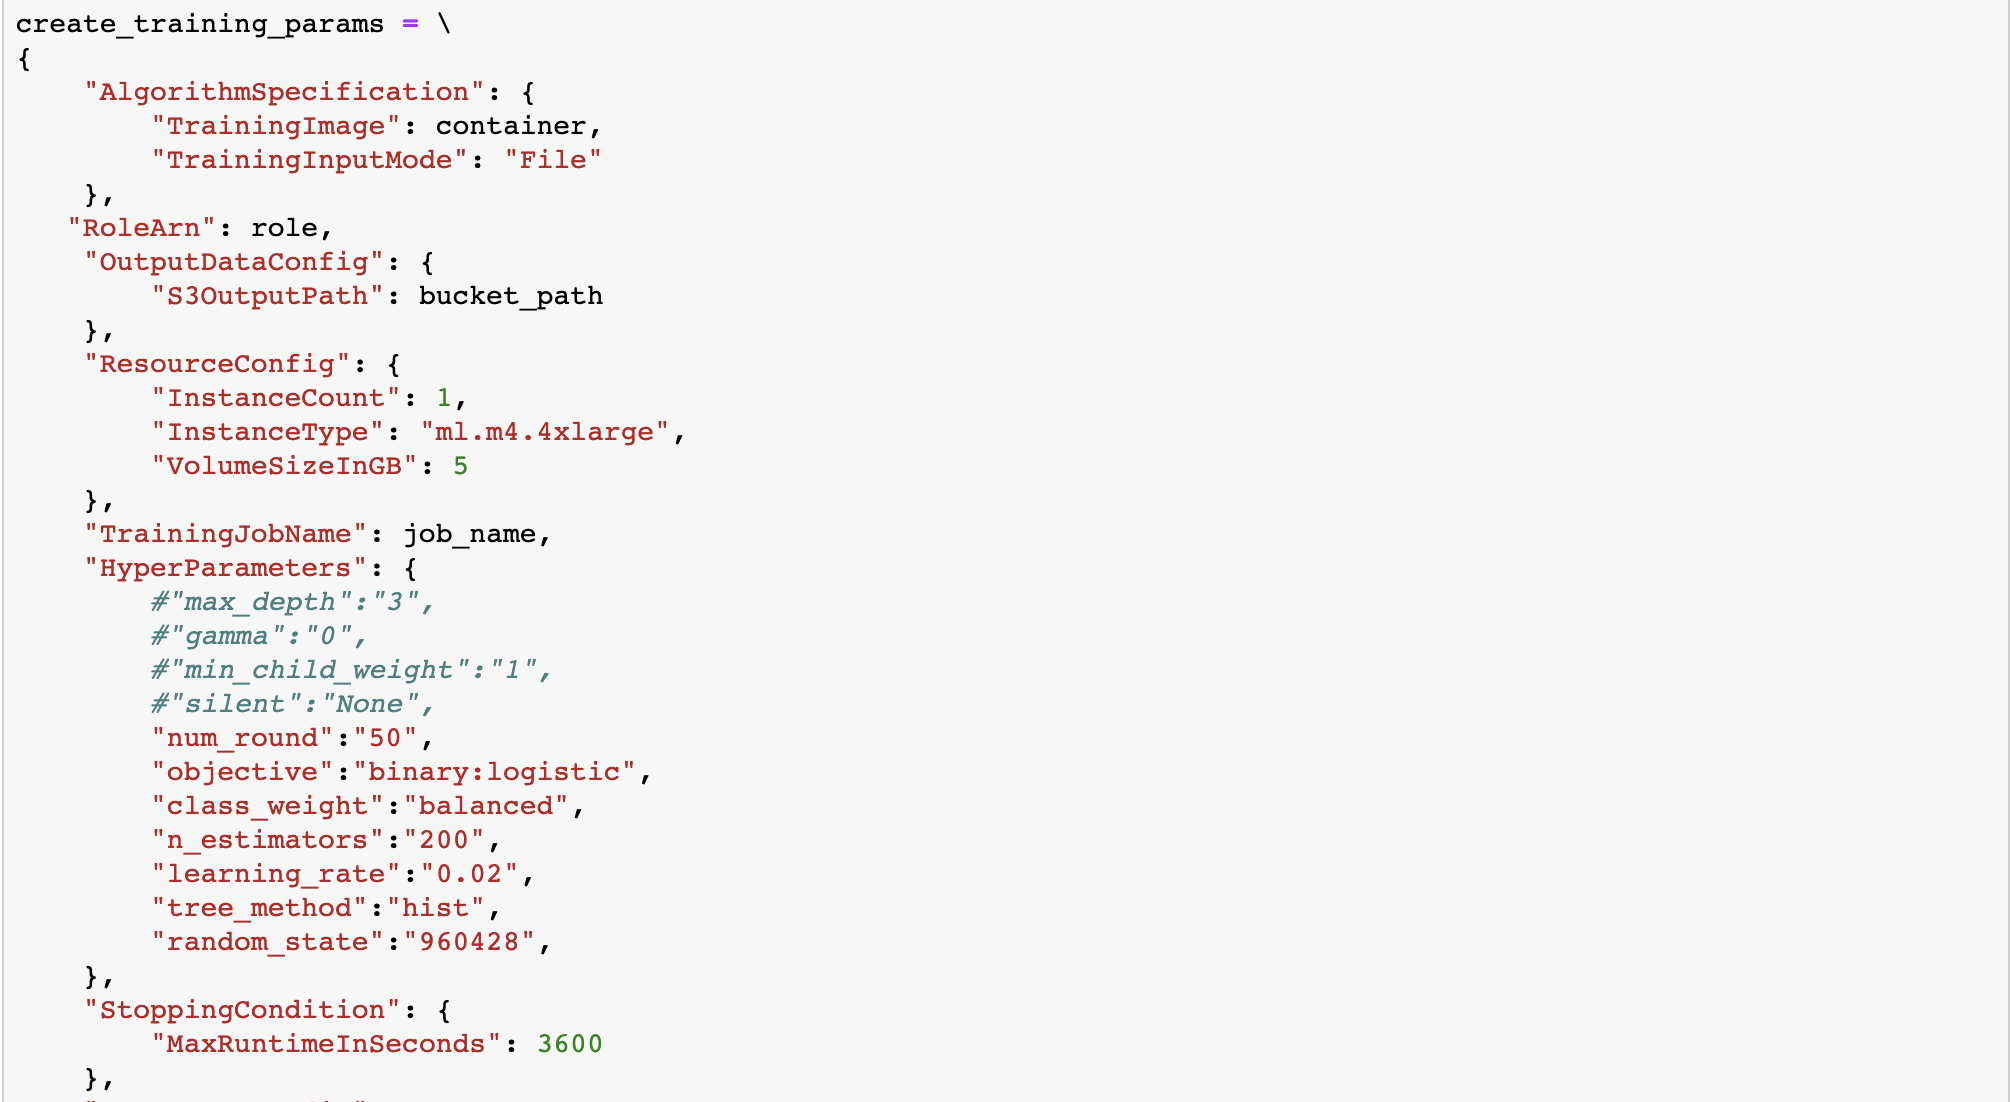
\includegraphics[width=1\linewidth]{confgi_1.png}
   \caption{configuring model part 1}
   \label{fig:confgi_1}
\end{minipage}%
\end{figure}
\noindent
\begin{figure}[H]
\centering
\begin{minipage}{1\textwidth}
  \centering
  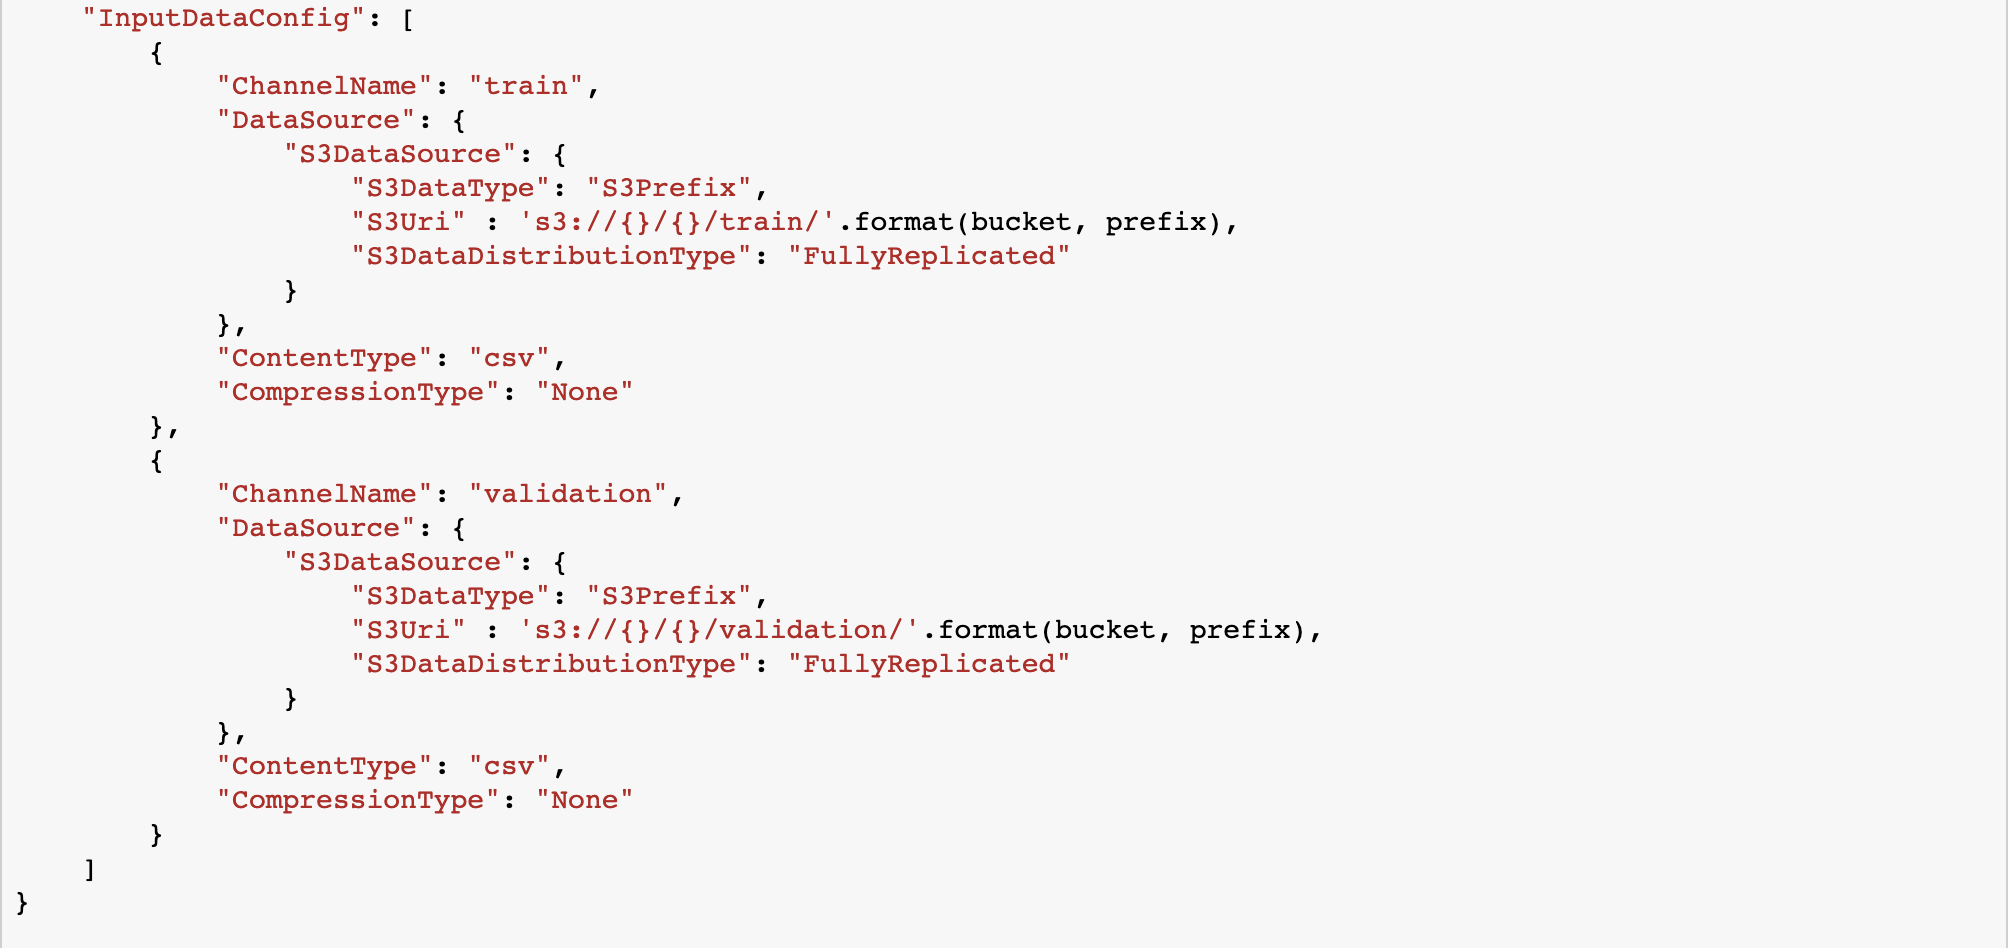
\includegraphics[width=1\linewidth]{confgi_2.png}
   \caption{configuring model part 2}
   \label{fig:confgi_2}
\end{minipage}%
\end{figure}
\noindent

\subsubsection{Begin train configuring model}
\begin{figure}[H]
\centering
\begin{minipage}{1\textwidth}
  \centering
  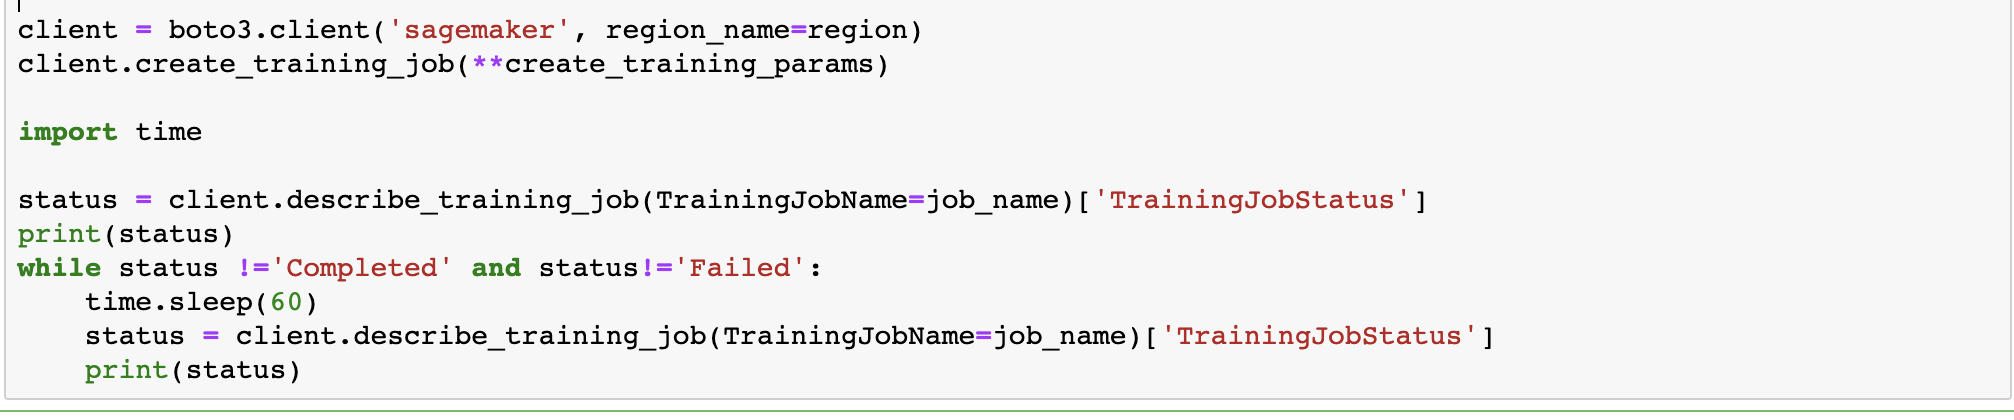
\includegraphics[width=1\linewidth]{train_model_2.png}
   \caption{Begin train configuring model}
   \label{fig:train_model_2}
\end{minipage}%
\end{figure}
\noindent




\newpage
\section{Deploy model with Batch Transformation}
We need one dataset \textit{testdataBatch.csv} in this step.

\subsection{Read in test data and specify batch output path}
See figure \ref{fig:batch_test_input}, firstly, we need to specify the batch input data, unlike train or validation dataset, we need to specify the name of test dataset for batch transformation. After that, we need to give the output path for batch transformation.

\begin{figure}[H]
\centering
\begin{minipage}{1\textwidth}
  \centering
  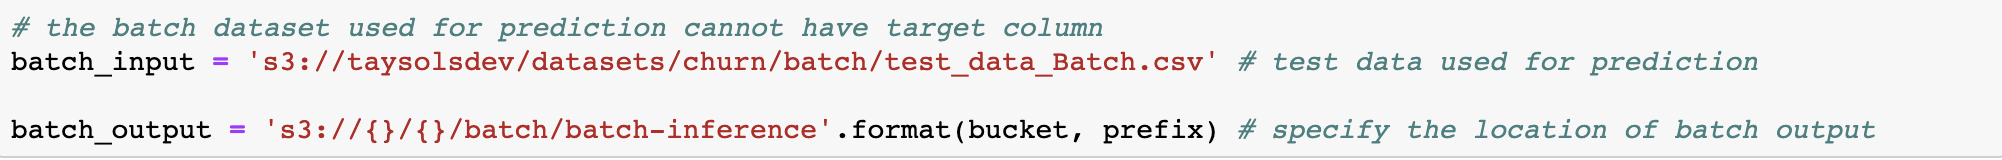
\includegraphics[width=1\linewidth]{batch_test_input.png}
   \caption{Read in test data for batch prediction}
   \label{fig:batch_test_input}
\end{minipage}%
\end{figure}
\noindent

\subsection{Run Batch Transform Job}
See figure \ref{fig:batch_transform_job}, to run a batch transform job, call the create\_transform\_job. method using the model that you trained before. \textit{initial\_instance\_count} :The initial number of instances to run in the Endpoint created from this Model. You can paste the following code in a cell in the Jupyter notebook. 

\begin{figure}[H]
\centering
\begin{minipage}{1\textwidth}
  \centering
  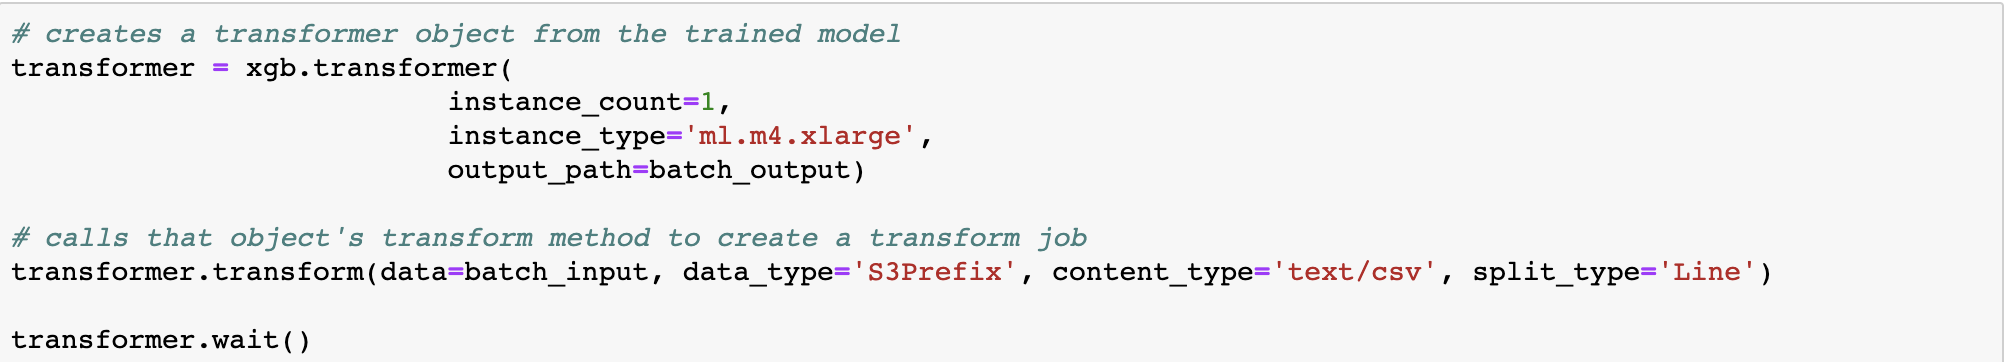
\includegraphics[width=1\linewidth]{batch_transform_job.png}
   \caption{Run Batch Transform Job}
   \label{fig:batch_transform_job}
\end{minipage}%
\end{figure}
\noindent



\newpage
\section{Validate Model Deployed with Batch Transform¶}
This step we need two datasets: the output prediction from batch transformation (\textbf{y\_pred}) and test dataset including true target values (\textbf{y\_test}).

\subsection{Read in Batch output file and test data}
See figure \ref{fig:read_in_testData}, to evaluate the model performance, firstly, we need to read in the batch predictions based on test dataset and true target values in test dataset. We can read in them use dataframe, note that we \textbf{must set \textit{header=None}}, otherwise we will loss the first row. 
\\
\noindent
Also, the \textit{test\_data\_Batch.csv.out} is different from \textit{test\_data\_Batch.csv}, the first one is batch output and the second one is batch input. they are located in two different data files.

\begin{figure}[H]
\centering
\begin{minipage}{1\textwidth}
  \centering
  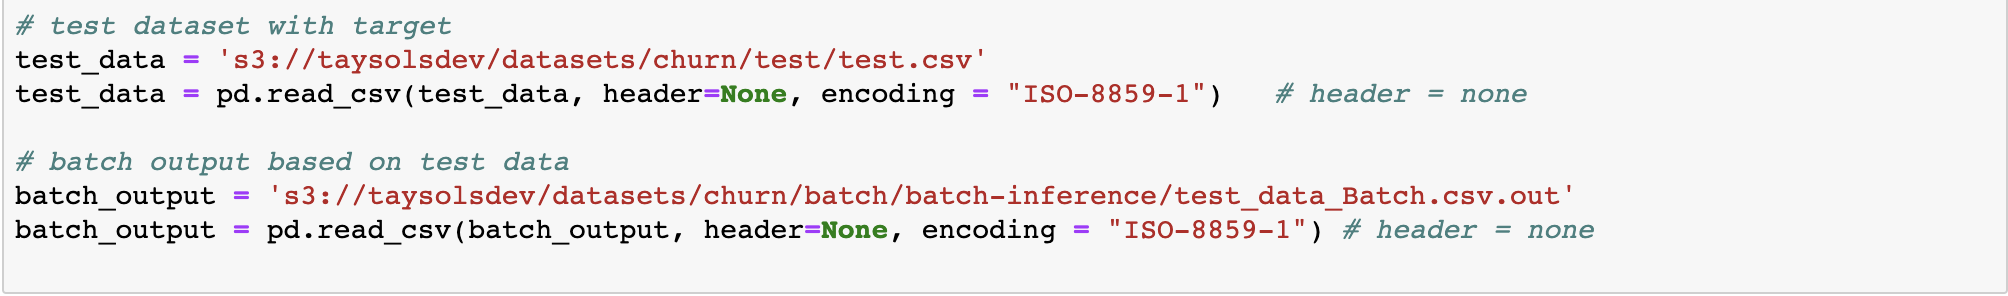
\includegraphics[width=1\linewidth]{read_in_testData.png}
   \caption{Read in Batch output file and test data}
   \label{fig:read_in_testData}
\end{minipage}%
\end{figure}
\noindent

\subsection{Model evaluation example}
See figure \ref{fig:read_in_testData}, the \textit{y\_test} is the first column in the \textit{test.csv}, and \textit{y\_pred} is the output dataset from batch transformation. Since we read them as dataframe, we can do any model evaluation calculation or plots using the general python code. In our binary classification example (threshold is 0.5):

\begin{figure}[H]
\centering
\begin{minipage}{1\textwidth}
  \centering
  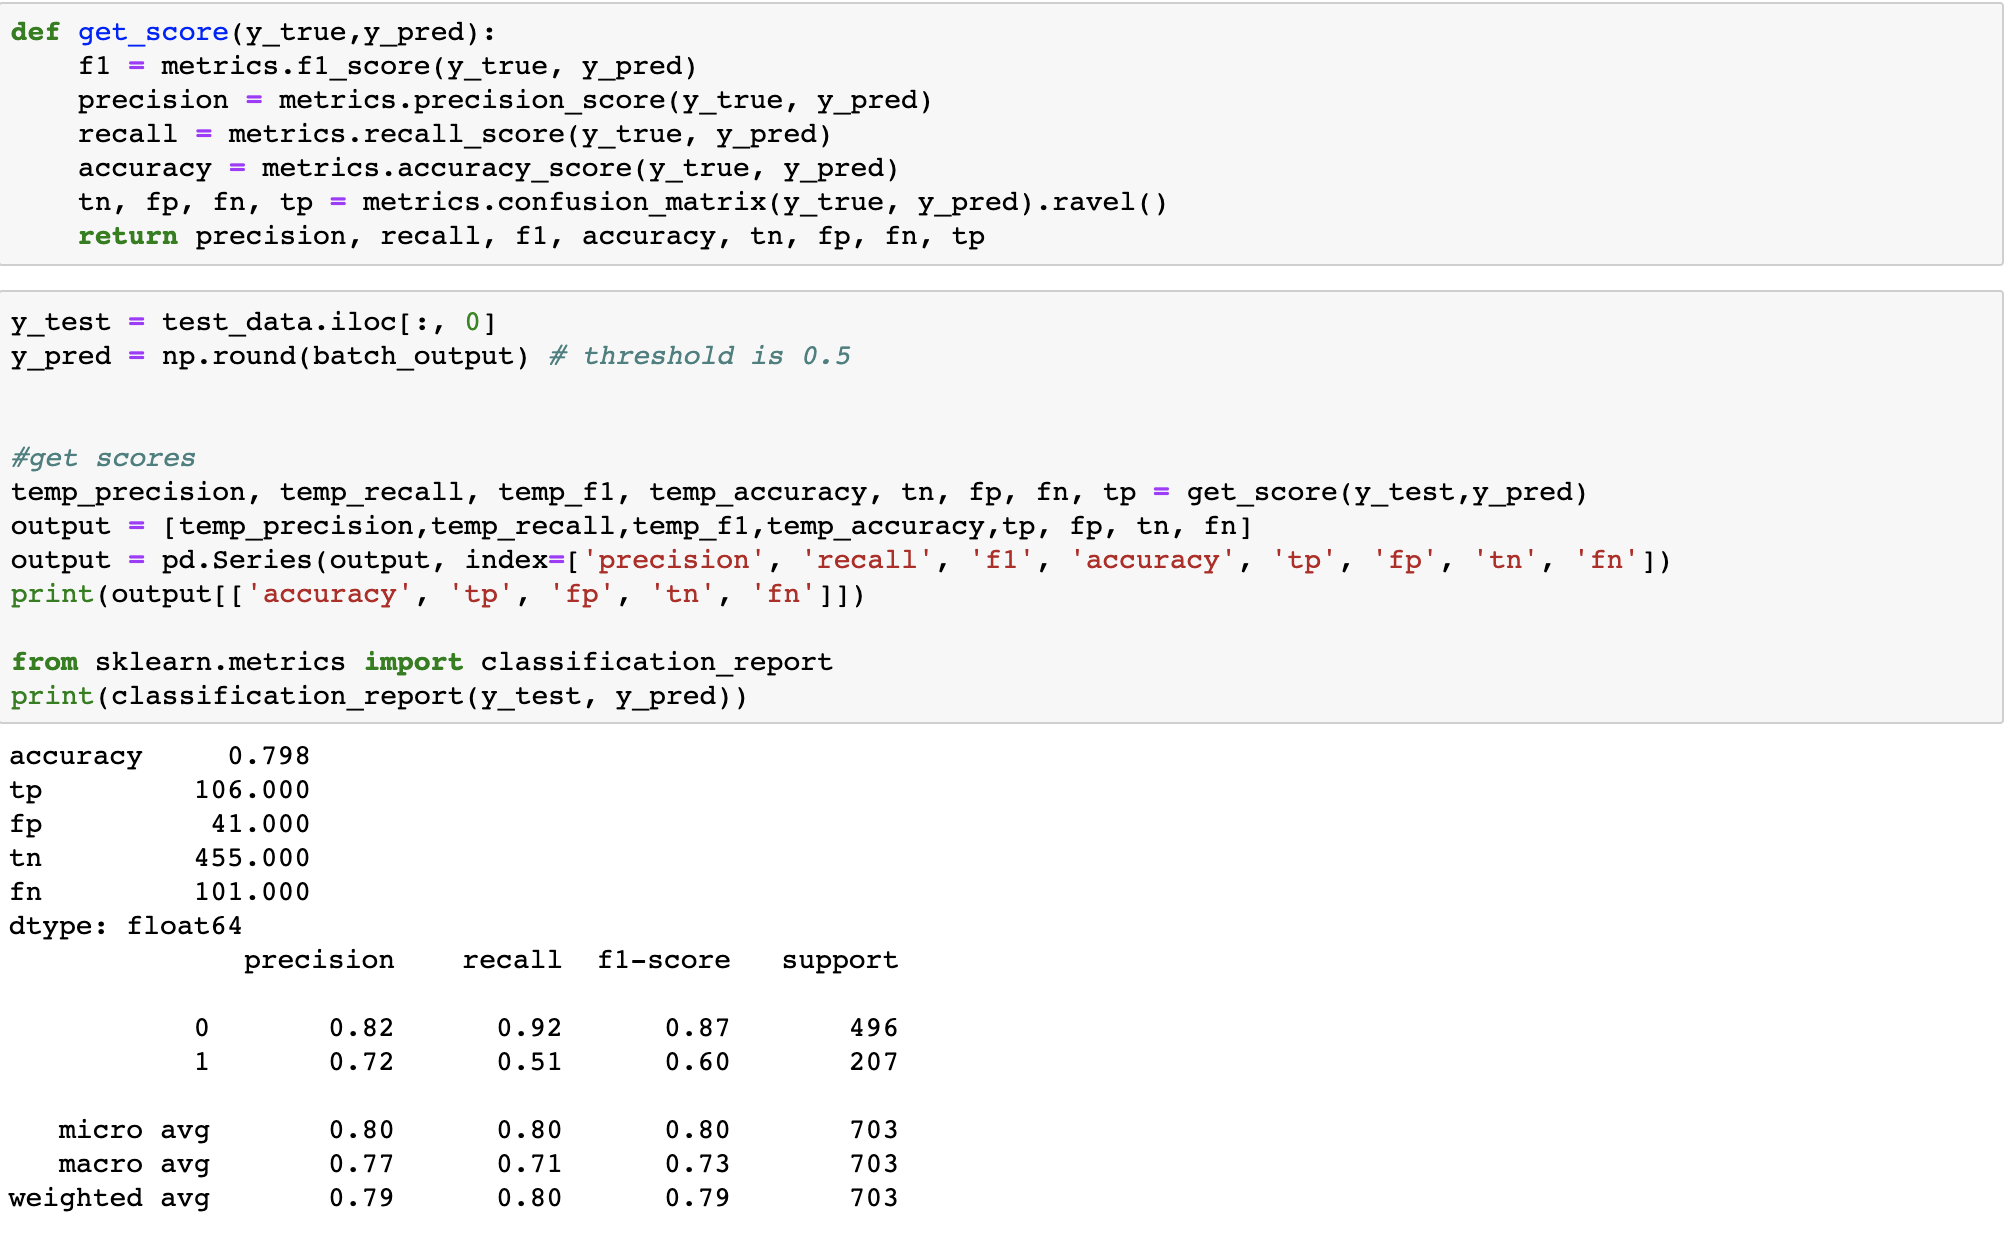
\includegraphics[width=1\linewidth]{validation_example.png}
   \caption{Model evaluation example}
   \label{fig:validation_example}
\end{minipage}%
\end{figure}
\noindent




\newpage
\section{Reference}

\begin{enumerate}
\item \url{https://github.com/awslabs/amazon-sagemaker-examples/blob/master/introduction_to_applying_machine_learning/xgboost_customer_churn/xgboost_customer_churn.ipynb}

\item \url{https://docs.aws.amazon.com/batch/latest/userguide/job_states.html}

\item \url{https://sagemaker.readthedocs.io/en/stable/overview.html#sagemaker-batch-transform}


\item \url{docs.aws.amazon.com/sagemaker/latest/dg/ex1-batch-transform.html}

\end{enumerate}






\setlength{\parskip}{1em}
\end{document}

